\chapter{Design and Experiments} \label{chap:experiments}
Summary of the experiment results and their details laid out in this section.
Neural network experiment logs are published online for more detailed examination, they are accessible by the URL provided in the corresponding footnotes.

\section{Training Specifications} \label{sec:trainspec}
Training for traditional machine learning used in this project is fallowing two-step approach.
At the first part hyper-parameters for the model is selected by cross-validation score then in the second part model is trained on the entire dataset with the selected hyper-parameters.
The final model then evaluated on the test set.

There are many artificial neural networks used in both in benchmarking and the model selection.
Weights of the networks initialized by random except for the transfer learning models.
The model used in the transfer learning experiments initialized with the weighs pre-trained on imagenet~\cite{imagenet} dataset.
Each architecture is trained using Adam~\cite{adam} optimizer with the default parameters ($\beta_1 = 0.9$ \& $\beta_2 = 0.999$).
I used a batch size of 64 for the training, and default learning rate of 0.001 that decayed by the factor of ten every time validation loss stagnates at the end of an epoch.
Each image in the dataset is downscaled to $224 \times 224$ shape and normalized to have values between 0 to 1.
Data augmentation is applied to minority class in the dataset to create a balanced dataset as explained in section \ref{sec:dataprocessing}.
Random cropping, changing saturation and horizontal flipping are set of augmentations chosen to create a balanced dataset.



\section{Benchmark Experiments}

\subsection{Random Forest Classifier and SVC}
Cross-validation results of the random forest classifier found the fallowing hyper-parameters achieves the best performance:

\begin{itemize}
    \item Number of trees: 500
    \item Information gain criteria: Gini
    \item Number of max features: Square root
    \item Bootstrap: allowed
\end{itemize}

Cross validation for the support vector machine classifier runs suggested the fallowing hyper-parameters will achieve the best metrics:

\begin{itemize}
    \item Regularization parameter: 10
    \item Kernel: rbf
    \item Polynomial degree: 3
    \item Kernel coefficient $\gamma$: scale
    \item Tolerance: 0.001
\end{itemize}

Confusion matrix of these classifiers evaluated on test data generated following results.

\begin{figure}[H]%
    \centering
    \subfloat[Random forest]{{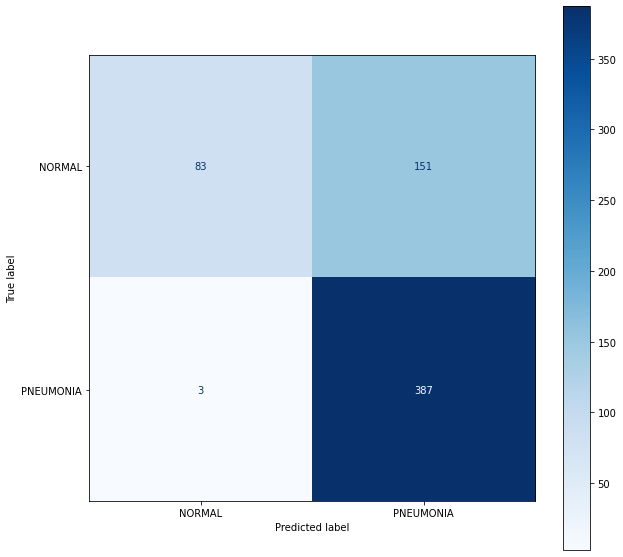
\includegraphics[width=.4\textwidth]{img/rf-confusion-matrix.png} }}%
    \qquad
    \subfloat[SVC]{{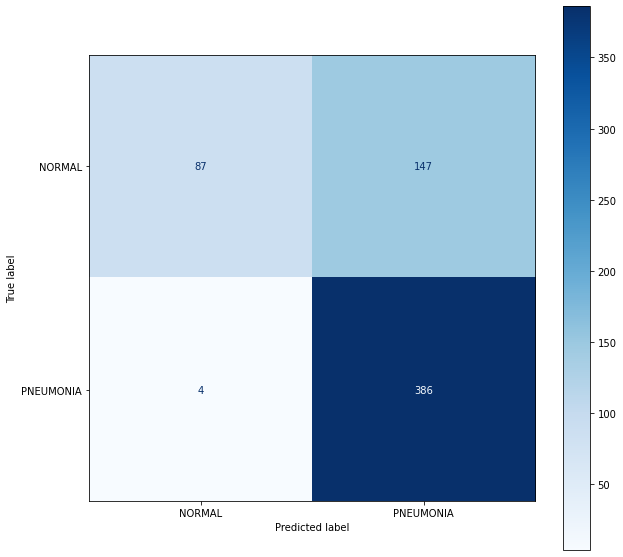
\includegraphics[width=.4\textwidth]{img/svm-confusion-matrix.png} }}%
    \caption{Confusion matrix of the classifiers.}%
    \label{fig:cmatrix}%
\end{figure}

It is clear from the amount of wrongly classified healthy patience X-ray, both of the models suffer from the imbalance effect.
This effect is slightly more dominant in the random forest classifier than the SVC, albeit performance of both models are similar.

\begin{table}[H]
    \centering
    \begin{tabular}{||c c c c c||} 
    \hline
    Classifier & Accuracy & Precision & Recall & f1\\ [0.5ex] 
    \hline\hline
    Random Forest & 0.7532 & 0.3547 & 0.9650 & 0.5187\\ 
    \hline
    SVC & 0.7580 & 0.3718 & 0.9560 & 0.5354\\
    \hline
    \end{tabular}
    \caption{Performance metrics for traditional machine learning algorithms.}
    \label{table:mlmetrics}
\end{table}



\subsection{AlexNet}
During the experiments for AlexNet and LeNet5 effect of the balanced dataset~\footnote{AlexNet Balanced: https://tensorboard.dev/experiment/7b6W0tdHQQ2RINGt6cYbrA/} is also compared to base dataset~\footnote{AlexNet Base: https://tensorboard.dev/experiment/PaBawCErSqG6zIef7JPq8g/} to measure the effectiveness of the data augmentation.
Figures used in AlexNet and LeNet5 annotated with balanced training/validation to reflect that balanced dataset is created with the data augmentation.
Base training/validation is used to refer base image data is used without any data augmentation.
Results from AlexNet was acceptable but given the loss values did not declined in the validation dataset suggest that ALexNet may have over-fitted the data.

\begin{figure}[H]
    \centering
    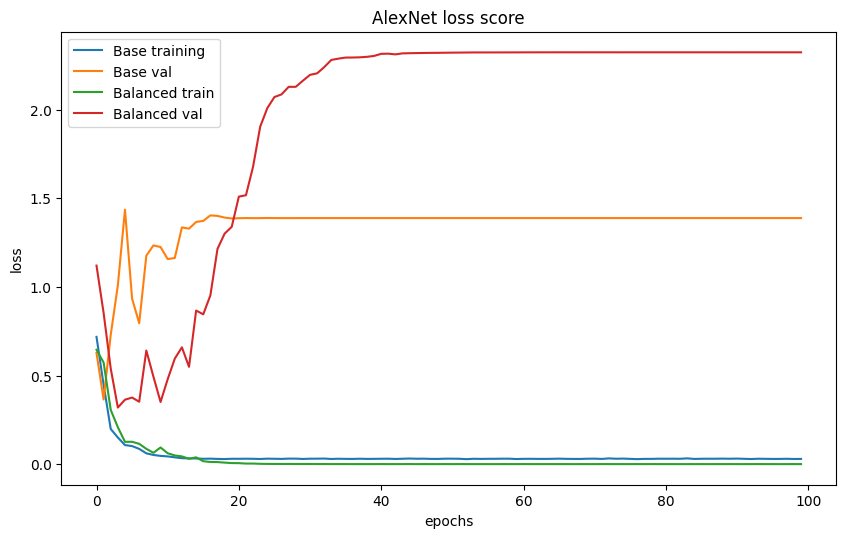
\includegraphics[width=.8\textwidth]{img/alexnetloss.png}
    \caption{}
    \label{fig:alexloss}
\end{figure}

Another important point is that convergence was very quick for this dataset. 
It is clearly visible in the charts that model converges in around first 30 epochs and remained unchanged for the rest of the training.

\begin{figure}[H]
    \centering
    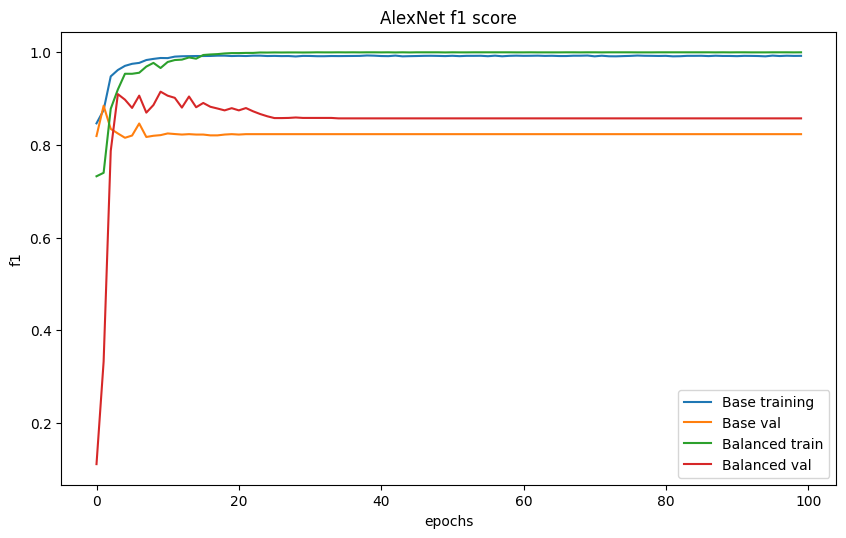
\includegraphics[width=.8\textwidth]{img/alexnetf1.png}
    \caption{}
    \label{fig:alexf1}
\end{figure}


\subsection{LeNet-5}
I was not able to train the LeNet5 model with the original model specification that utilizes hyperbolic tangent function (tanh).
This was partially expected as tanh activation function is not able to pass the gradient flow very well when the initialization is not favourable.
This effect is mentioned in section \ref{sec:gradients} and as such, I have replaced the activation function with the ReLu activation function for my implementation.
Similar to AlexNet, LeNet5 also displayed a possible sign of over-fitting when loss did not decline on the validation dataset.

\begin{figure}[H]
    \centering
    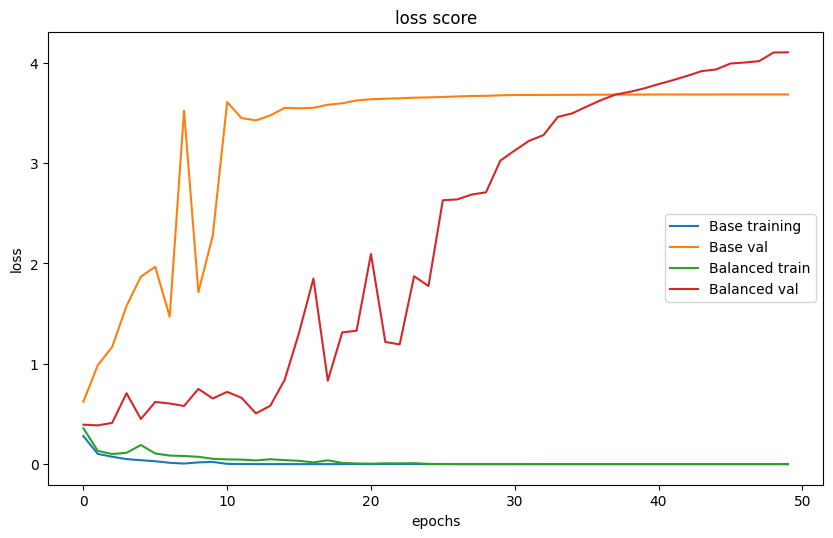
\includegraphics[width=.8\textwidth]{img/lenetloss.png}
    \caption{LeNet5 loss metrics}
    \label{fig:lenetloss}
\end{figure}

\begin{figure}[H]
    \centering
    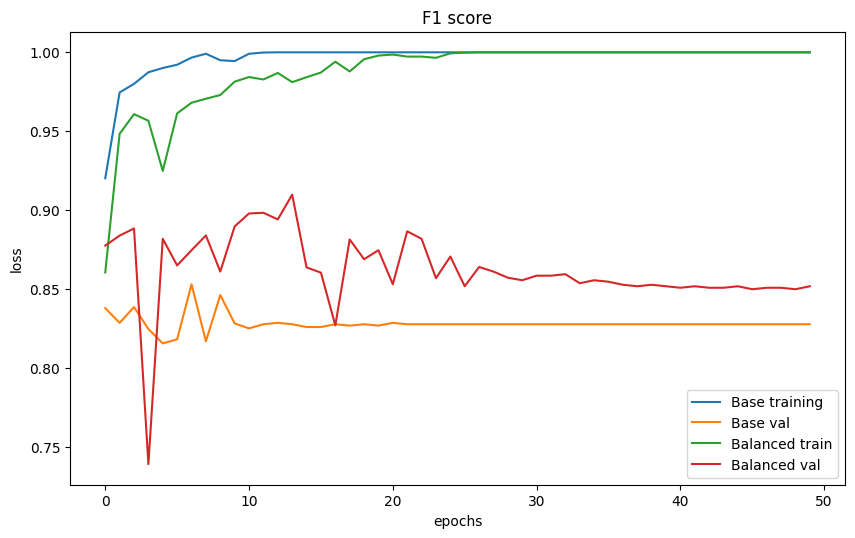
\includegraphics[width=.8\textwidth]{img/lenetf1.png}
    \caption{LeNet5 f1 metrics}
    \label{fig:lenetloss}
\end{figure}

LeNet5 performance was slightly below AlexNet's on the holdout data, yet it is still a considerable performance given the algorithm is the oldest one among the neural networks.

\subsection{VGGNet}
Performance of this model~\footnote{VGGNet Base: https://tensorboard.dev/experiment/IbsPnocxSMKqNjmdJ3CdpA/}~\footnote{VGG Balanced: https://tensorboard.dev/experiment/ABd8GrKdSXyzHgNPDngeEw/} is the worst among all of the model I tried.
Disappointing performance didn't change with the different random initialization.
However, training and validation loss suggested good training by declining in both training and validation data, accuracy metric was below random guess.

\begin{figure}[H]
    \centering
    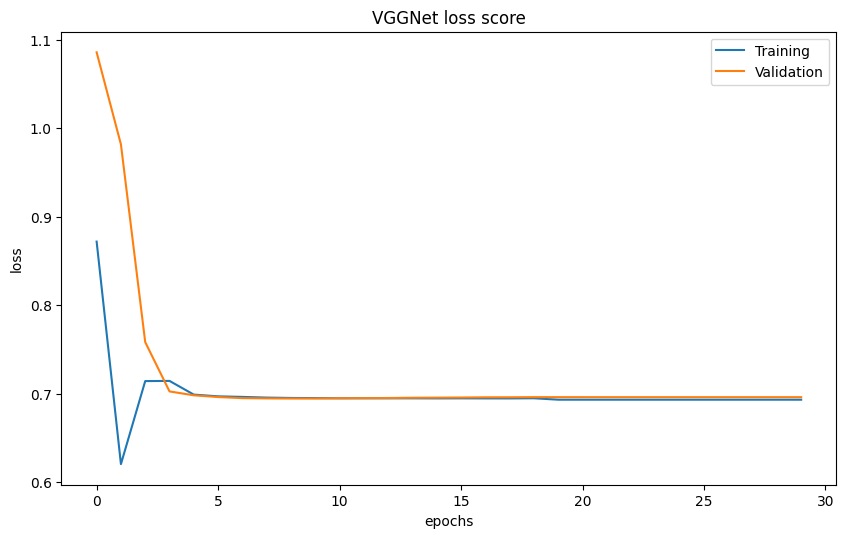
\includegraphics[width=.8\textwidth]{img/vggnetloss.png}
    \caption{}
    \label{fig:vggloss}
\end{figure}

\begin{figure}[H]
    \centering
    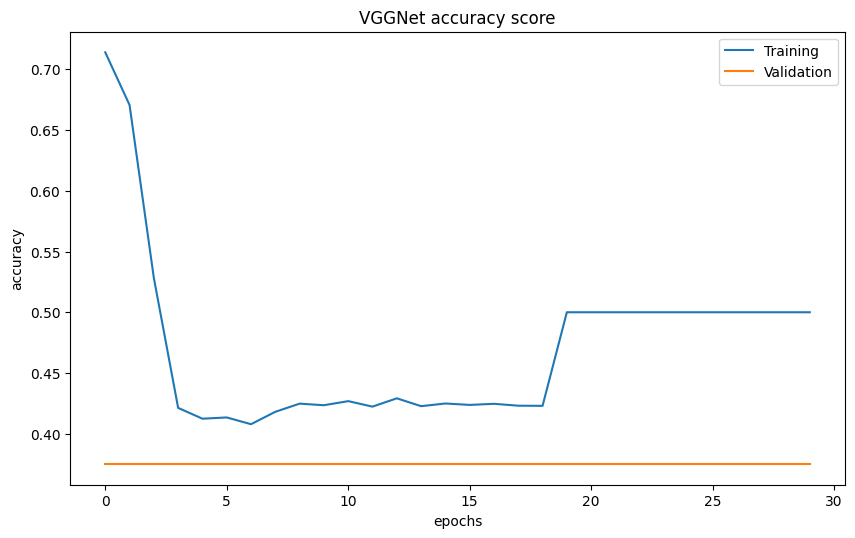
\includegraphics[width=.8\textwidth]{img/vggnetaccuracy.png}
    \caption{}
    \label{fig:vggacc}
\end{figure}

% vggnet https://tensorboard.dev/experiment/IbsPnocxSMKqNjmdJ3CdpA/
% vgg balanced https://tensorboard.dev/experiment/ABd8GrKdSXyzHgNPDngeEw/

\section{Transfer Learning}
I was very skeptical when adopting transfer learning to pneumonia detection because of the fundamental difference in the type of images in the imagenet compare to the project images.
In this implementation weights in the convolutional part of the model initialized with the pre-trained VGGNet model from imagenet dataset.
Convolution layer weights in this network are kept frozen during the training and allowed only fully connected layers at the end of the model to be trained.
To my surprise, this approach worked considerably well. Achieving $\approx 77 \%$ in accuracy and $\approx 87 \%$ f1 on validation data. 

\begin{figure}[H]
    \centering
    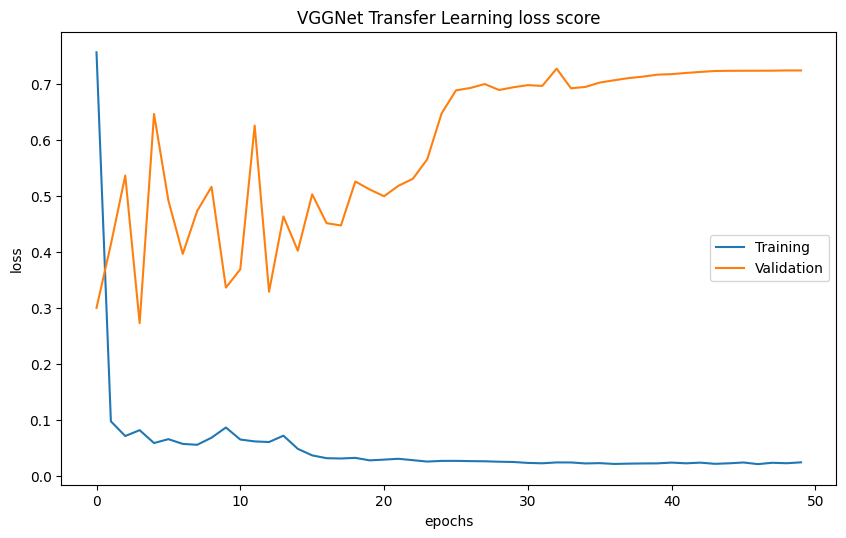
\includegraphics[width=.8\textwidth]{img/vggnettfloss.png}
    \caption{}
    \label{fig:vggtfloss}
\end{figure}

\begin{figure}[H]
    \centering
    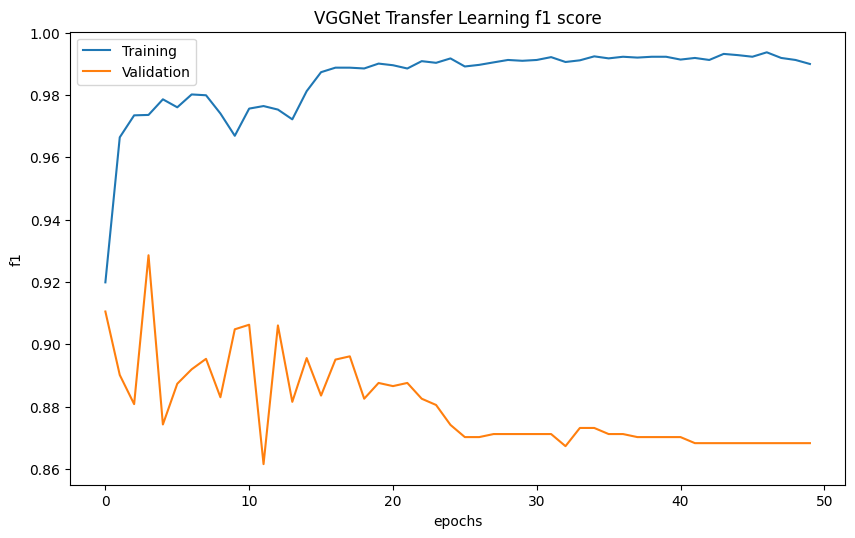
\includegraphics[width=.8\textwidth]{img/vggnettff1.png}
    \caption{}
    \label{fig:vggtff1}
\end{figure}

Although transfer learning has proven to be a viable method to increase model performance, fine-tuning attempts on transfer learning was unsuccessful~\footnote{https://tensorboard.dev/experiment/QRbFzlgwSGaf0lu5LLRSzA/}.
After unfreezing top convolutional block layers and training the model, performance decreased to below 0.4 in the validation accuracy with a f1 score of zero.
% \begin{figure}[H]
%     \centering
%     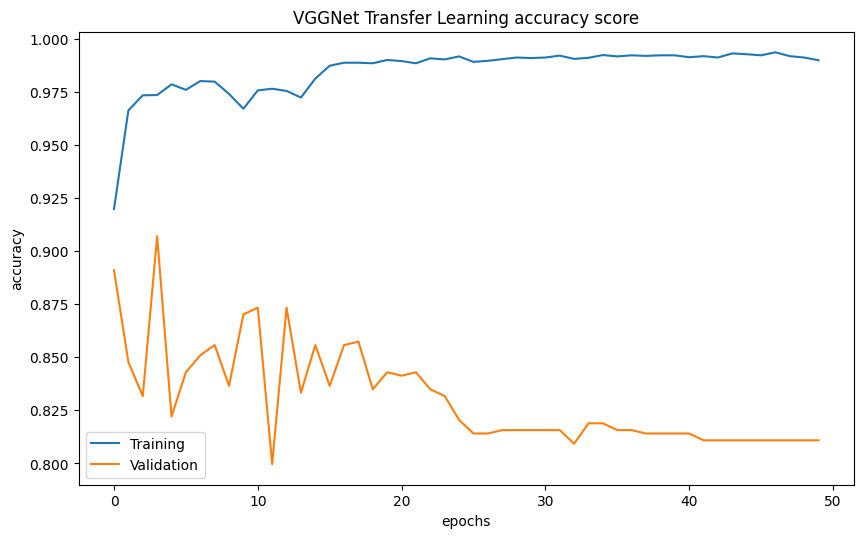
\includegraphics[width=.8\textwidth]{img/vggnettfaccuracy.png}
%     \caption{}
%     \label{fig:vggtfacc}
% \end{figure}
% vgg https://tensorboard.dev/experiment/VxxyXkn6TaSMrgKnSP1low/
% vgg-balanced https://tensorboard.dev/experiment/c1zSx6N0QviARqCVIq3QMw/

\section{Custom Neural Network Architecture}
After experimenting~\footnote{https://tensorboard.dev/experiment/BDwUXqGgSVWA8Ieawcb3Rg/} with a randomly chosen number of layers best combination I discovered is an architecture with ten convolution layers followed by batch normalization and max-pooling layer. 
In final experiments showed using two convolutional layers fallowed by batch normalization layer and max-pooling layer like a convolutional block is the best optimal choice for this architecture.

\begin{figure}[H]
    \centering
    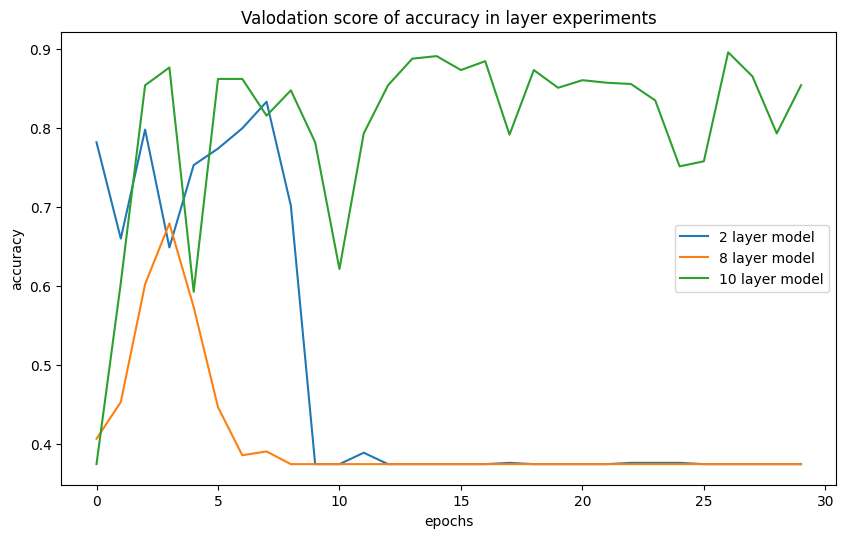
\includegraphics[width=\textwidth]{img/layerexpaccuracy.png}
    \caption{}
    \label{fig:layerexpacc}
\end{figure}

Immediately after this experiments, the same number of layers are maintained to determine the performance of the type of the convolution layer on the dataset.
For the same number of layers, I replaced the convolutional layers with the depthwise separable convolutional layers~\footnote{https://tensorboard.dev/experiment/aA2SgzCNTXWXK7kWMhyJNg/}.
Depthwise separable convolutional layers work by performing a depthwise convolution first then mixing that with the pointwise convolution.
The result shows that convolutional layers perform better than depthwise convolutional layers whit the same layer numbers and other convolution properties set equally.

\begin{figure}[H]
    \centering
    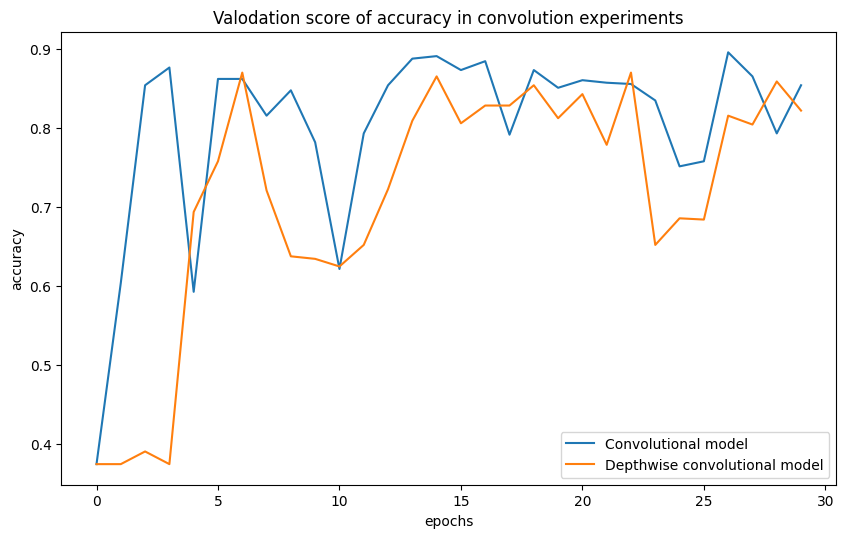
\includegraphics[width=.8\textwidth]{img/deptoconvexpaccuracy.png}
    \caption{}
    \label{fig:depttoconvacc}
\end{figure}

Lastly, I have started experiments~\footnote{https://tensorboard.dev/experiment/x8d0woI6Q7SpKo8zc0ZbSQ/} to observe the effect of regularization at the fully connected layers.
Varying levels of dropout rate applied to dense layers to fine-tune the regularization level that best suits this architecture. Results show that the best level of dropout rate as 30\%, albeit dropout rates in the effect of the dense layers change very little the performance scores of the model.


\section{Interpreting Model Decisions}
Application of GradCAM~\cite{cam} provided valuable insight into understanding the features and parts of the images that lead to a certain type of prediction.
In the case of images with the pneumonia presence models usually focused on the lung or lung segments which were expected.
However, occasionally some predictions were based on regions that consist of bones that suggested that search for a better model should continue.

\begin{figure}[H]%
    \centering
    \subfloat{{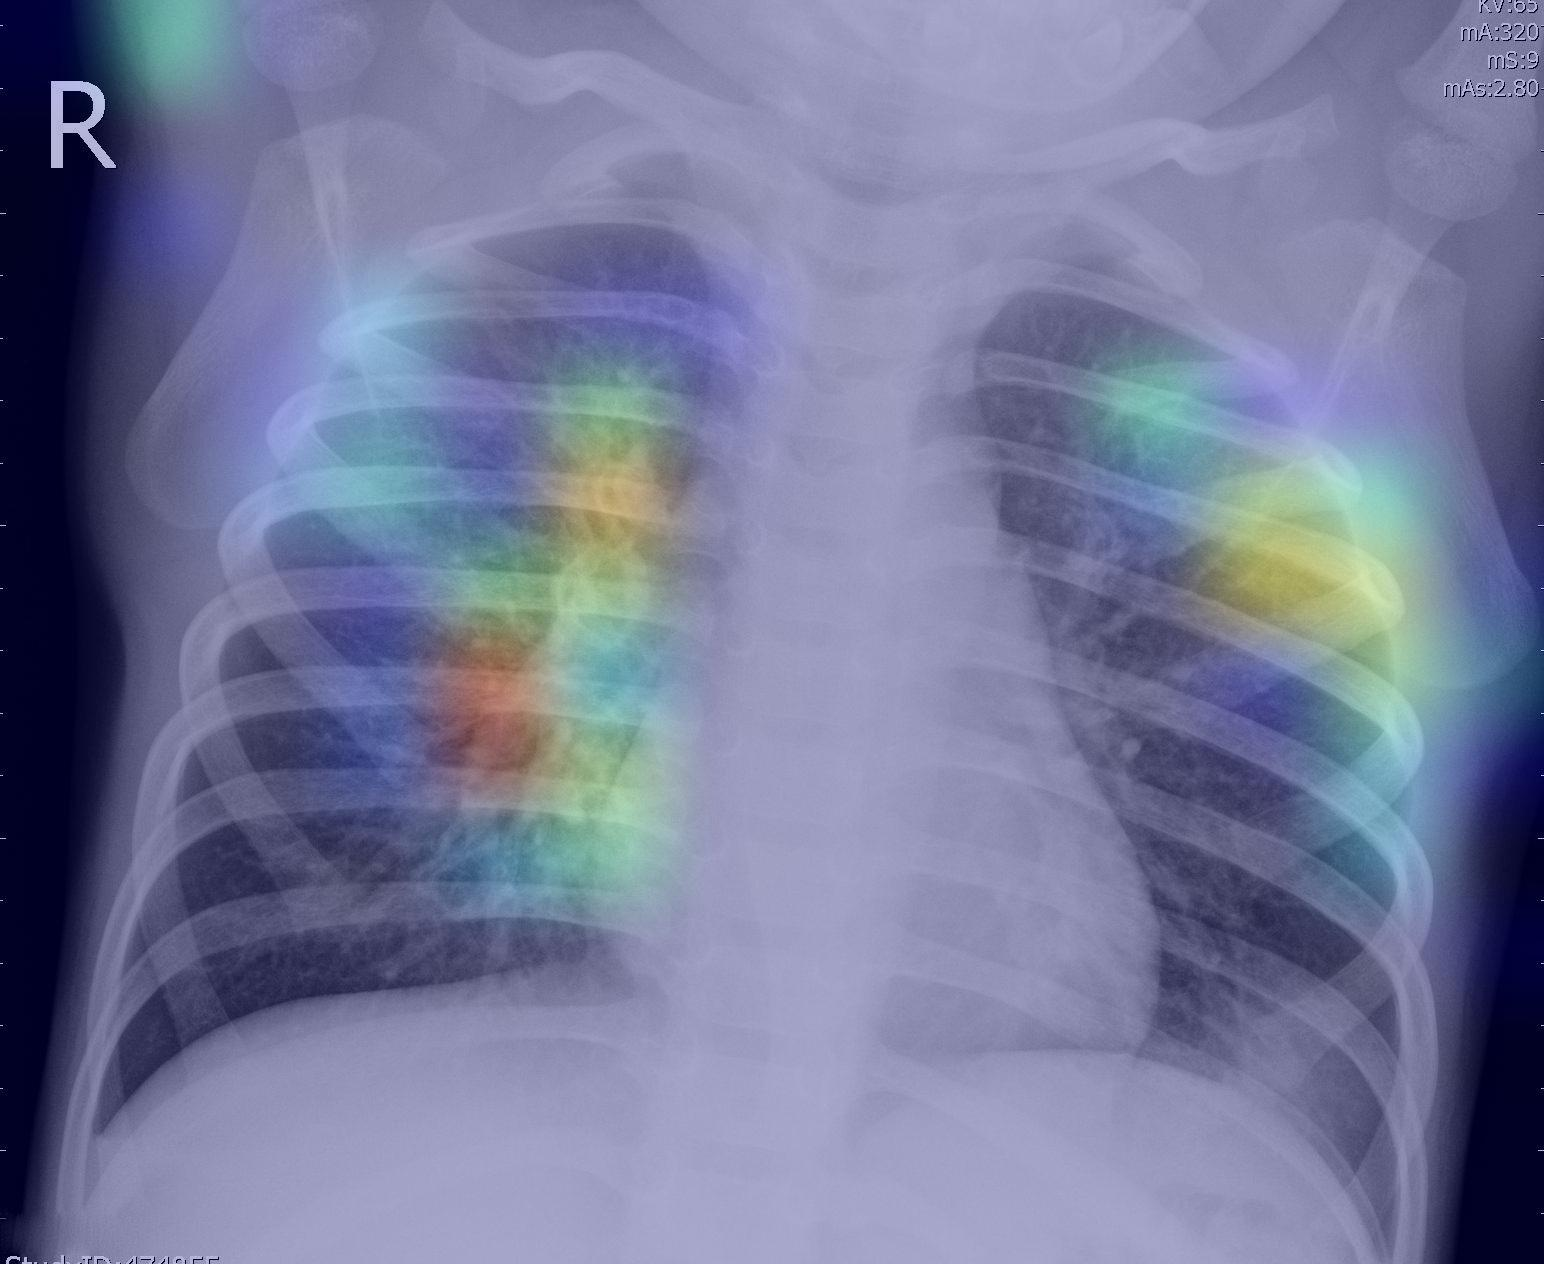
\includegraphics[width=.4\textwidth]{img/pnue38.jpg} }}%
    \qquad
    \subfloat{{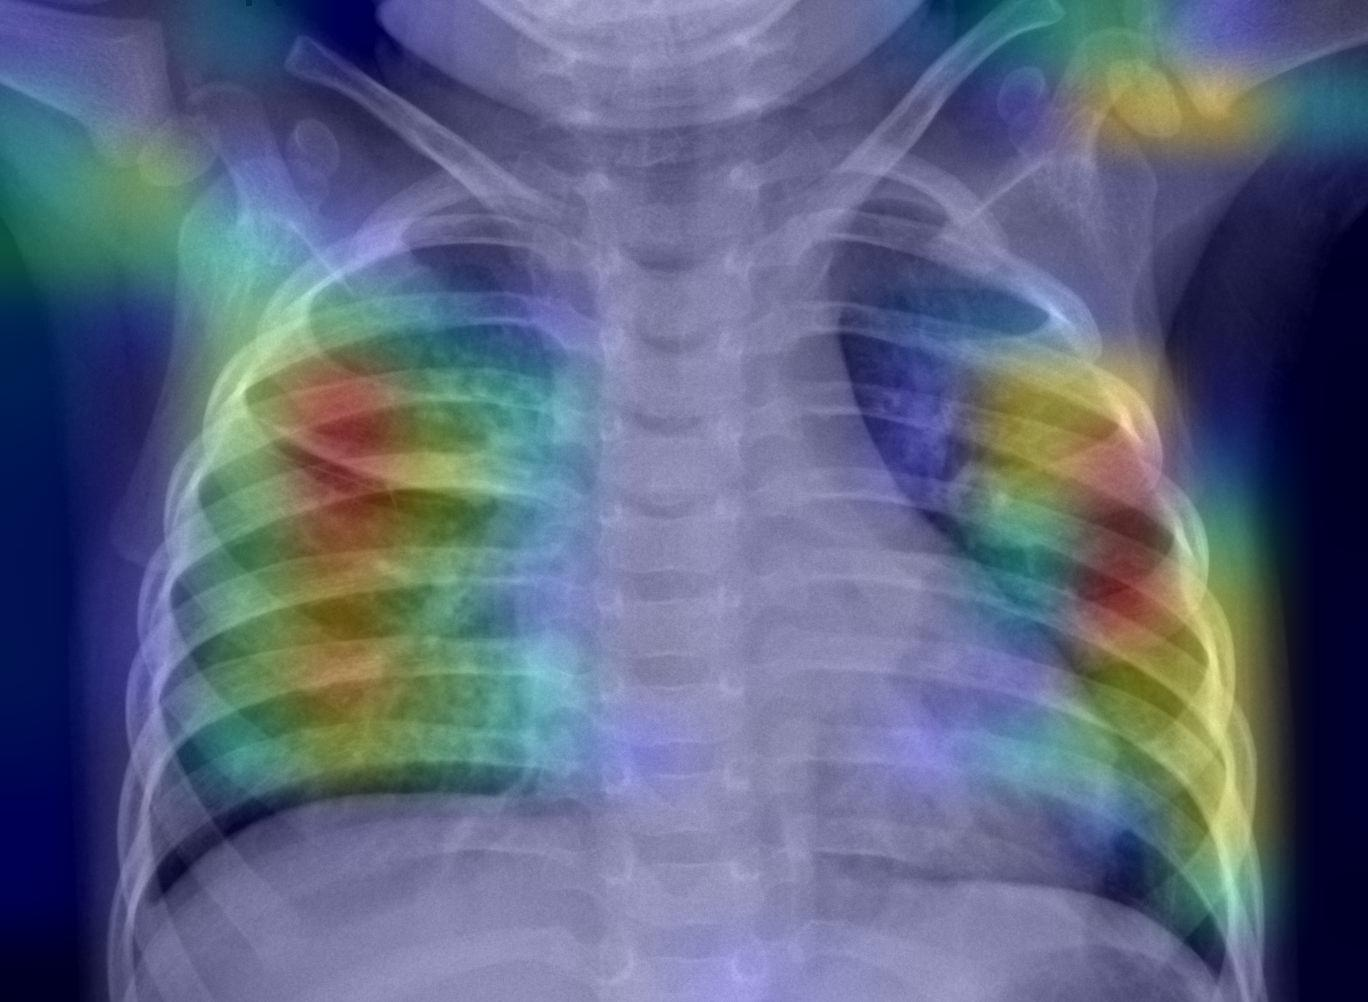
\includegraphics[width=.4\textwidth]{img/pnue42.jpg} }}%
    \caption{GradCAM result of the images with pneumonia diagnosis.}%
    \label{fig:campnue}%
\end{figure}

It was also noteworthy that in the case of absence of pneumonia X-rays models tend to focus on features like background or bone structures.
One such example is the figure \ref{fig:camnormal}, that model gives emphasis on the background above shoulders and curved parts of the ribs of the patient.

% \begin{figure}[H]%
%     \centering
%     \subfloat[Random forest]{{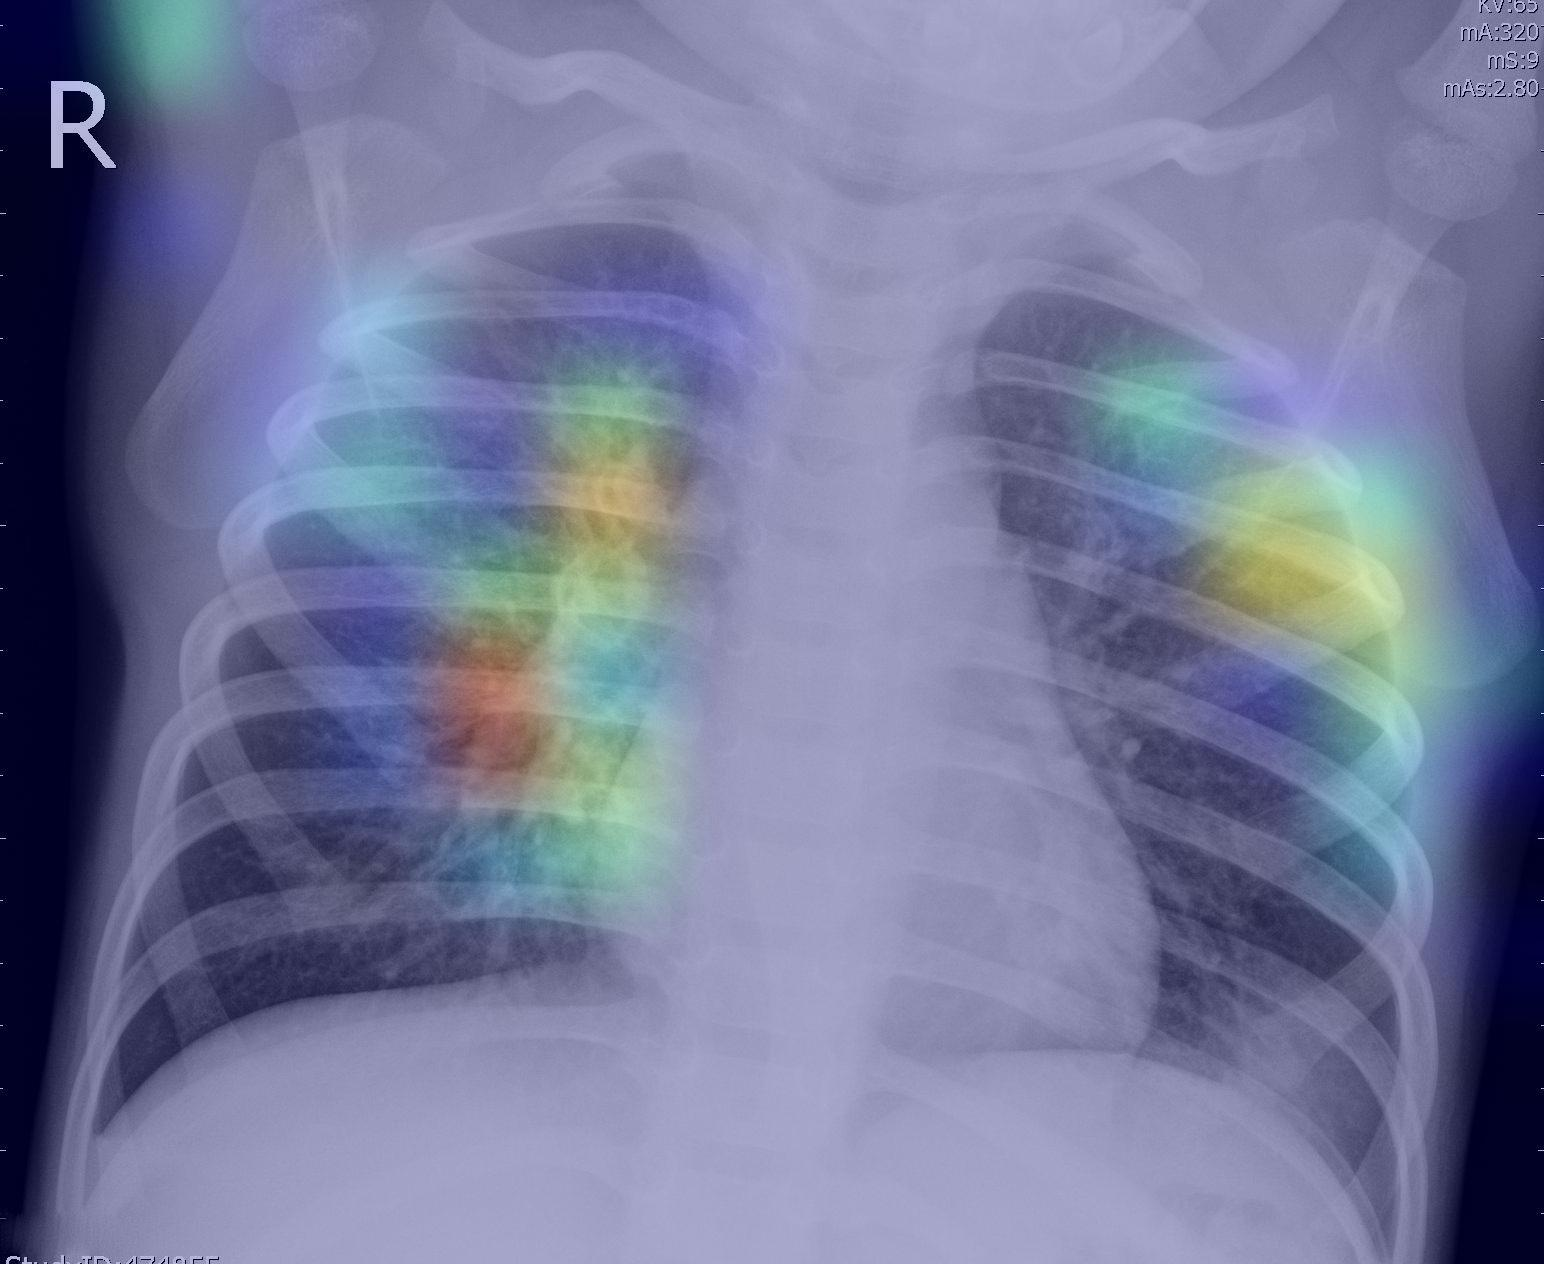
\includegraphics[width=.4\textwidth]{img/pnue38.jpg} }}%
%     \qquad
%     \subfloat[SVC]{{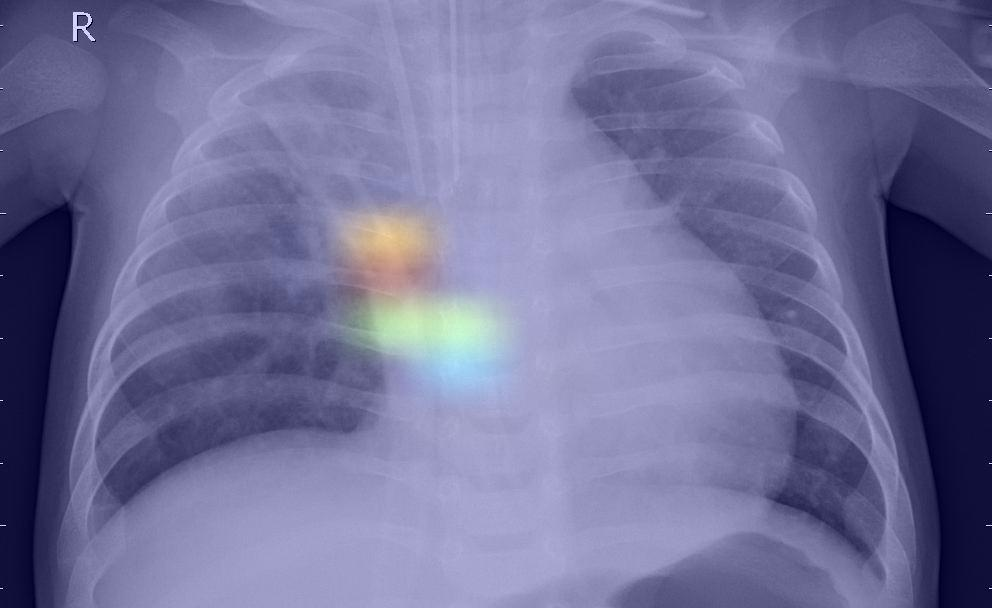
\includegraphics[width=.4\textwidth]{img/pnue27.jpg} }}%
%     \caption{GradCAM result of the images with pneumonia diagnosis.}%
%     \label{fig:campnue}%
% \end{figure}

% \begin{figure}[H]%
%     \centering
%     \subfloat[Random forest]{{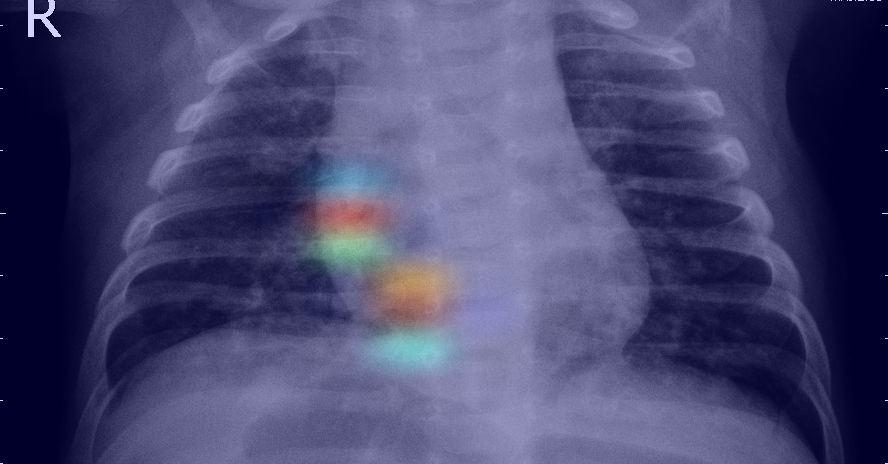
\includegraphics[width=.4\textwidth]{img/pnue25.jpg} }}%
%     \qquad
%     \subfloat[SVC]{{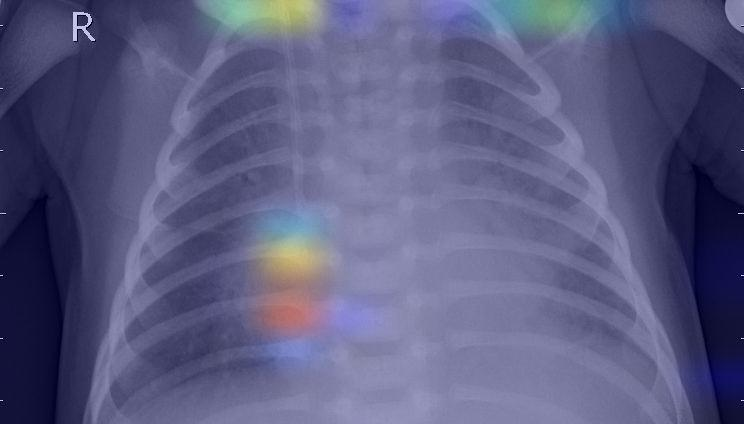
\includegraphics[width=.4\textwidth]{img/pnue22.jpg} }}%
%     \caption{GradCAM result of the images with pneumonia diagnosis.}%
%     \label{fig:campnue}%
% \end{figure}

\begin{figure}[H]%
    \centering
    \subfloat[Stand alone heatmap]{{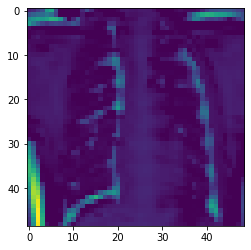
\includegraphics[width=.35\textwidth]{img/heatmapnormal.png} }}%
    \qquad
    \subfloat[Overlayed heatmap on image]{{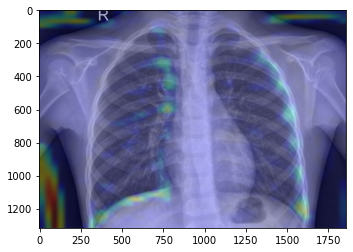
\includegraphics[width=.45\textwidth]{img/normalimg.png} }}%
    \caption{GradCAM result and heatmap of the image without pneumonia diagnosis.}%
    \label{fig:camnormal}%
\end{figure}

Model interpretability tool, in this case, is valuable for the decision making in which models to promote to production, especially in the case of selecting between models that have very close performance metrics.

% base (https://tensorboard.dev/experiment/p2mkNoLORACZlCXL2UQRbg)
% augmented (https://tensorboard.dev/experiment/dmQIbMeJQtqF70MhQQqySA)